\begin{flushright}
	
\end{flushright}\chapter{Literature Review}
\label{cha:2_literature}
\parskip=0ex

\section{Cyber Attack on Firmware and Remote Firmware Update for Embedded Device}
\label{sec:1_issues}

In 2011, cyber attack on embedded battery controller firmware could possibly cause a security hazard such as overheated the battery and made it catch fire~\cite{batteryfirmware}. Embedded battery controller is usually used in Li-Ion and Lithium Polymer batteries. These types of battery are used in embedded devices, therefore the overheating battery can cause embedded devices be permanently broken.

\sloppy In 2013, Cui et al.~\cite{conf/ndss/2013} demonstrated how firmware update process can be exploited. The vulnerability allow the attacker to inject malicious firmware modifications into the embedded device. Cui et al. successfully exploited the third-party libraries in HP printer firmware images and injected malicious modification into the library. Their experiment result proved the capabilities of the running-malware in printer, such as: network reconnaissance, data exfiltration, and propagation to general purpose computer or other embedded device types. 

The other cyber attack that can be done in firmware update process is replay attack. During the firmware update process, attacker can duplicate the firmware binary from the vendor server and make the victim device check the unnecessary firmware update. The redundant checking process will drain the victim device battery. To resist replay attack, ~\cite{iotsecurity} use timestamp and nonce mechanism. Embedded device does not need to check the duplicate firmware update within the small interval of time by checking the timestamp of the request.

In the firmware update process, adversary can intersect the firmware binary from the vendor. Using reverse engineering algorithm, attacker can modify the firmware or inject malicious code and send it to the victim device. To keep the integrity and the authenticity of the firmware, firmware binary can be digitally signed by vendor using its private key. After downloading the firmware binary from the vendor's repository, embedded device can validate the digital signature using the attached public key. Once the firmware is validated, the update process is started.

There are currently two methods to update the device's firmware, manual and automatic process. Manual process is vulnerable and not efficient, because user needs to manually download the firmware binary and install it to embedded device. Downloaded firmware integrity and authenticity can not be confirmed by un-experienced end user nor by the embedded device because it is manually downloaded and installed. On the other hand, automatic update over the Internet needs secure channel to ensure the integrity and authenticity of the firmware. Firmware Over The Air (FOTA) is typically used for automatic firmware update, general FOTA process is described in Figure ~\ref{fig:1_fota}. This automatic update process (remote firmware update) will update the latest firmware binary to the targeted device without manual operation.

\begin{figure}[H]
	\begin{center}
		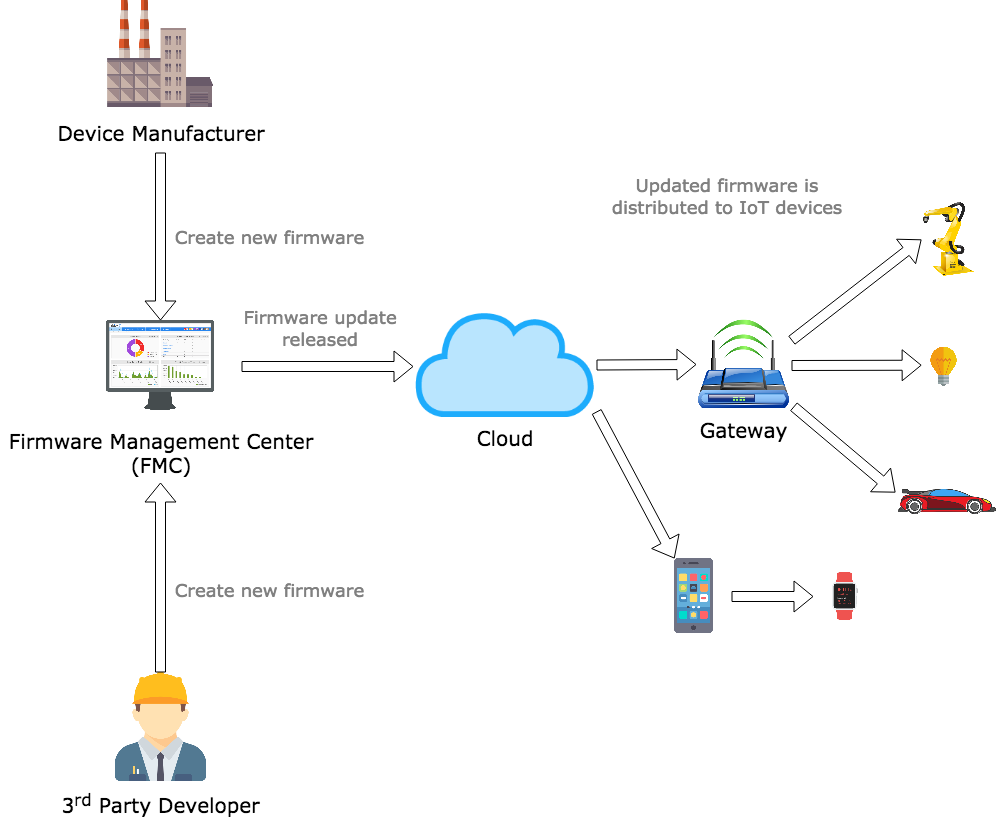
\includegraphics[width=1.0\textwidth]{figures/img_firmware_update_fota.png}
		\caption{Firmware Over The Air (FOTA) process diagram} 
		\label{fig:1_fota}
	\end{center}
\end{figure}

Remote firmware update uses two methods in its process, push and pull method. While push method is applicable for resource constrained device, pull method is more practical for more powerful with stable connection device~\cite{securefota}. Both methods use client-server architecture, in the push method, vendor repository as the server sends the firmware binary as chunks to the device as the client. After receiving the whole firmware binary, client will notify the server aby sending an error or success message. If there is no error, client can do the firmware update. In pull method, vendor repository as a server will provide a url to download the firmware binary to the gateway as the client. Once the whole firmware binary is downloaded, the error or success notification message will be sent back to the server. Then, client can do the firmware update if the download is successful.

\section{Blockchain}
\label{sec:2_blockchain}

Based on Satoshi Nakamoto~\cite{Satoshi}, blockchain was originally created for peer-to-peer electronic cash payment transaction based on cryptographic proof instead of trust (to third party, such as Bank). Satoshi Nakamoto proposes a solution to prevent the double-spending problem in peer-to-peer network without a trusted third party. Each transaction data in the blockchain network is verified, time-stamped and linked with the previous data in the form of chained hash (proof-of-work). By doing so, blockchain technology can create a record that cannot be changed without redoing the hash-based proof-of-work.

Bitcoin's proof-of-work uses Adam Back's Hashcash~\cite{hashcash} which is originally created to limit email spam and denial of service attack (DDoS). The block generation process in Bitcoin uses Hashcash as its proof-of-work. In order for a block to be accepted by network participants, miners must complete a proof-of-work which covers all of the data in the block. Miner is any node that lends their computational resource in order to secure the network and is rewarded with some bitcoin. The first miner who finds the nonce and successfully creates the new block will be rewarded.

Bitcoin implement the proof-of-work ~\cite{proofofwork} by incremental nonce in the block until a value (nonce) is found, this nonce together with the transaction data must give block's hashed value (using SHA-256) the required zero bits. The example of how Bitcoin's proof-of-work iterates nonce is shown in Figure ~\ref{fig:2_proofofwork}. In this example, the required zero value is 3 and it must be in the beginning of the hash value. Total of 4251 hashes iteration is needed in this case, which is not a very hard computation (most computer can achieve at least 4 million hashes per second). That is why Bitcoin automatically varies the difficulty to keep a roughly constant rate of block generation. The difficulty of this proof-of-work is adjusted so as to limit the rate at which a new block can be generated in the network for every 10 minutes. Due to the very low probability of successful generation of a block, this makes it unpredictable which worker computer (miner) in the network will be able to generate the next block.

\begin{figure}[H]
	\begin{center}
		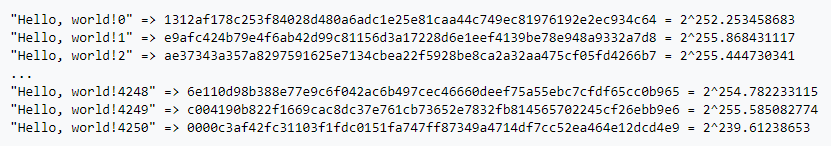
\includegraphics[width=1.0\textwidth]{figures/proofofwork.png}
		\caption{Iterating nonce that make hashes value begin with a number of zero value~\cite{proofofwork}} 
		\label{fig:2_proofofwork}
	\end{center}
\end{figure}

After the correct nonce and its corresponding hash value is found in the mining process, chaining algorithm is depicted in Figure ~\ref{fig:3_blockchainning}. Each block's hash value contains the hash value of previous block. As all blocks in the ledger are chained with its previous block, any modification on the value of any block will affect the whole blocks structure in the network. This mechanism makes blockchain tamper-proofing, means that no one can modify nor tamper a transaction once it is validated and recorded into blockchain.

\begin{figure}[H]
	\begin{center}
		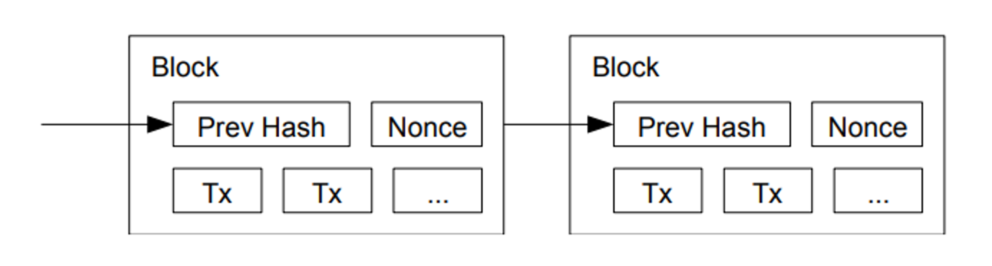
\includegraphics[width=1.0\textwidth]{figures/block-chainning.png}
		\caption{Nakamoto's chaining block diagram~\ref{fig:3_blockchainning}} 
		\label{fig:3_blockchainning}
	\end{center}
\end{figure}

\section{Skiplist}
\label{sec:3_skiplist}

\textit{Skiplist} was first described in 1989 by William Pugh ~\cite{skiplistOriginate}. Skiplist is a data structure that allows fast search within an ordered sequence of elements ~\cite{wiki:skiplist}, fast search is possible by skipping over a few element rather than searching linear number of steps. The structure of a skiplist is shown in Figure ~\ref{fig:4_skipliststructure}. As an example, the search process to find the fifth node, the skiplist firstly traverse a link of width 1 at the top level. Now four more steps are needed, but the next span on this level is too large (10), so it will drop one level to level 3. The algorithm once again traverse one link of width 3. Since the next step of width 2 is skpping too far (becomes 6), instead of traversing in the same level, it will drop down to the bottom level. Lastly the skiplist will traverse the final link of width 1 to reach the fifth link (target).

\begin{figure}[H]
	\begin{center}
		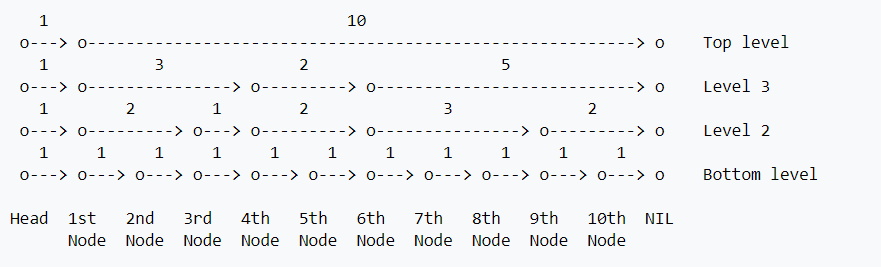
\includegraphics[width=1.0\textwidth]{figures/skiplistSearch.png}
		\caption{Skiplist structure with span between two same-level nodes~\ref{fig:4_skipliststructure}} 
		\label{fig:4_skipliststructure}
	\end{center}
\end{figure}

Based on how the insertion process, there are two types of skiplist. In deterministic skiplist, user needs to define how the insertion process needs to be done. For example J. Ian Munro~\cite{deterministicSkiplist} defined "1-2 skiplist", "1-2 skiplist" structure requires either one or two nodes of height (h-1) exist between any two nodes of height {\emph{h}} ({\emph{h}} > 1). The deterministic skiplist structure is shown at Figure ~\ref{fig:5_deterministicSkiplist}

\begin{figure}[H]
	\begin{center}
		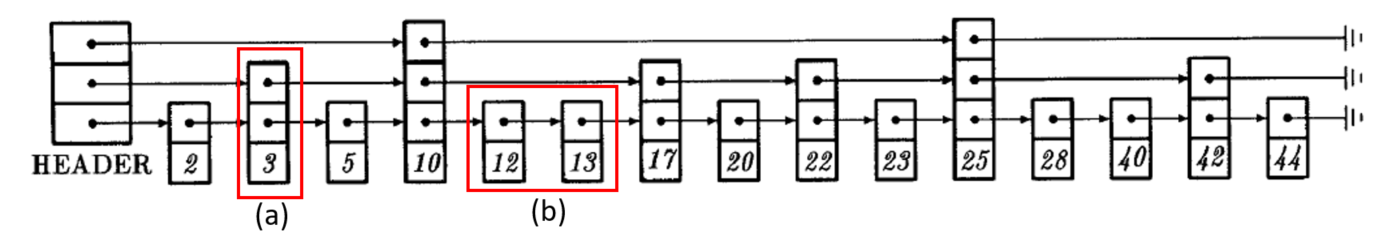
\includegraphics[width=1.0\textwidth]{figures/deterministicSkiplist.png}
		\caption{(a) There is a node with height of two between two nodes with height of three. (b) There are two nodes with height of one between two nodes of height of two~\cite{deterministicSkiplist}} 
		\label{fig:5_deterministicSkiplist}
	\end{center}
\end{figure}

On the other hand, a randomized skiplist defines the new node height based on probabilistic of a coin toss. It will add the height of the newly inserted node until the coin-toss lands on tail or the height reach the maximum-defined-height. The randommess makes the average insert and update cost for the skiplist is low. Randomized skiplist can achieve simple implementation but requires larger storage. 

\section{Skipchain}
\label{sec:4_Skipchain}
One of the key characteristic of blockchain is the traceable asset. It allows all blockchain's participants know where the asset come from and how it change overtime. However, to verify an asset will require user's device to be online, connected to the Internet and to pay bandwidth and power costs to maintain the connectivity with multiple nodes on blockchain network~\cite{Skipchain}. User can to join as a full node, maintaining a mirror copy of the entire blockchain to verify or trace an asset. As an option, user can join as a lightweight node and download partial amount of the entire blockchain data from connected full node. However, it is difficult for low power, limited storage and limited connection device to join the blockchain network even as lightweight node.

Joining a blockchain network as a lightweight node is not without risk, a compromised full node can isolate the connected lightweight node using a "fake" view of blockchain. The lightweight node can do a secure verification by synchronizing with multiple full node, but the compromised full node can achieve it goals by deceiving the isolated lightweight node during the "offline" state. The blockchain node remain vulnerable to isolation attack because the fundamental problem is that the current blockchain can never be validated in any absolute ways, but only relative to the perspective from another node.

To tackle this issue, Chainiac~\cite{chainiac} introduced skipchain, a novel cryptographic blockchain structure that adapts the skiplist idea by adding long-distance links both forward and backward in time as illustrated in Figure ~\ref{fig:6_skipchainStructure}. When Chainiac creates new block, it will create additional hash link to farther backward in time. On the same time, Chainiac also creates long-distance forward link via collective signatures~\cite{cosigning}. With long-distance forward and backward link, skipchain technology becomes cryptographically traversable in both directions. 

\begin{figure}[H]
	\begin{center}
		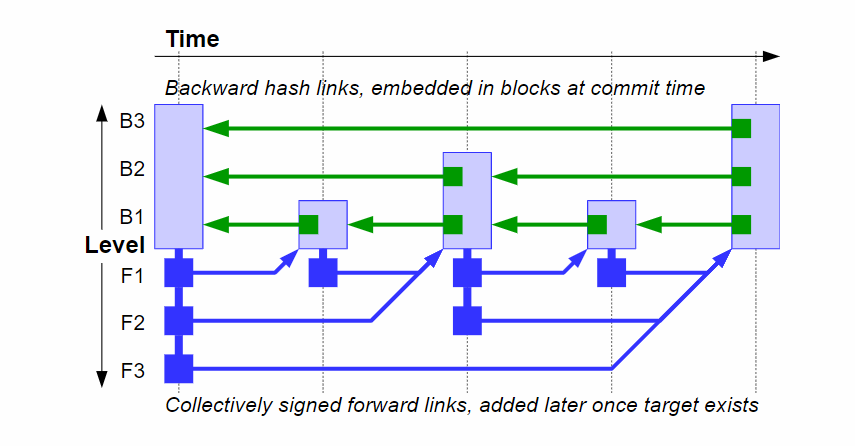
\includegraphics[width=1.0\textwidth]{figures/skipchainStructure.png}
		\caption{Skipchain structure~\cite{chainiac}} 
		\label{fig:6_skipchainStructure}
	\end{center}
\end{figure}

Using this skipchain characteristic, node as a client can efficiently prove the correctness of a transaction anywhere in time with respect to other party reference point on the blockchain, in a logaritmic number of steps, regardless of which node has a more up-to-date data view of the blockchain~\cite{Skipchain}. For example, a gateway in a smart home environment wants to show a new firmware update to a connected IoT device. In this case, the IoT device has limitations to connect to the Internet and to synchronize with the other node. The IoT device can not store partial part of the blockchain data due to its limited storage. The gateway can simply sends to the IoT device a small number of collectively signed forward links through a peer-to-peer connection to prove securely that the new firmware updates is indeed on the blockchain. 

\section{Blockchain-based Firmware Update Framework}
\label{sec:5_proposedFramework}

In this section, previous researches on the firmware update mechanism for embedded devices based on blockchain infrastructure are introduced. Lee et al.~\cite{lee} introduced the blockchain-based firmware verification and update schemes for embedded devices in IoT environment. Lee et al. mentioned that excessive network traffic may occur when large number of embedded devices downloading the latest firmware simultaneously from a dedicated firmware update server. This problem leads Lee et al. to utilize blockchain network concept, where a device can request a firmware update from a decentralized peer-to-peer network.

\sloppy In~\cite{lee} architecture, embedded device acted as full node in the blockchain network which was difficult to be implemented in real world scenario. Because the embedded devices with low-power, limited storage and limited connection to the Internet are difficult to maintain connection with the other node in blockchain network. It is also not possible for the embedded device to store growing blockchain data. Moreover, when there are many kind of embedded device with different requirement of firmware, it will take a long time to make the download request because this scheme used pull-method. In result, this scheme might not efficient for heterogeneous IoT ecosystem.

Boudguiga et al.~\cite{boudguiga} investigated that it was possible to use blockchain infrastructure to provide firmware update to several embedded devices belonging to different manufacturer. This scheme relied on trusted node in the blockchain to validate an update innocuousness before its transmission to the end objects. The trusted node checks that the new update does not contain bugs and resist to known attack.

There are two architectures introduced by~\cite{boudguiga}. In the first architecture, each vendor was expected to provide at least one worker node in the blockchain network. An embedded device could periodically pull the blockchain by random picks the node and check the firmware version. The mentioned trusted node takes place in the second architecture as a refinement from the first architecture. The trusted node directly receives new firmware binary from the vendor, then notifies the corresponding embedded devices after the validation process completed. The corresponding device can download the valid firmware binary and do the firmware update.
